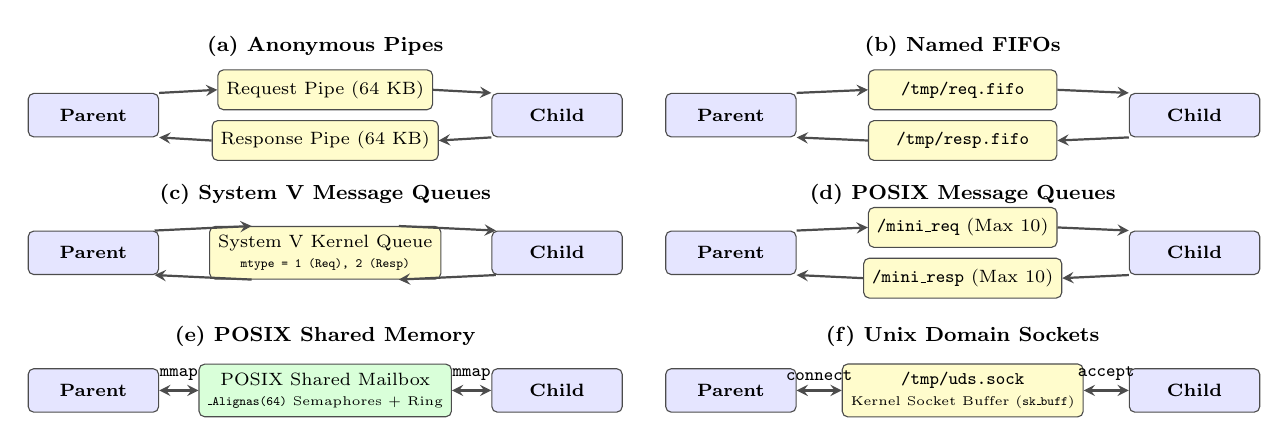
\begin{tikzpicture}[
    scale=0.92, every node/.style={transform shape},
    proc/.style={draw=black!70, fill=blue!10, rounded corners=2pt, font=\scriptsize\bfseries, minimum width=1.8cm, minimum height=0.6cm, align=center},
    buffer/.style={draw=black!70, fill=yellow!20, rounded corners=2pt, font=\scriptsize, minimum width=2.6cm, minimum height=0.55cm, align=center},
    shmbuf/.style={draw=black!70, fill=green!15, rounded corners=2pt, font=\scriptsize, minimum width=3.0cm, minimum height=0.55cm, align=center},
    arr/.style={->, >=stealth, thick, draw=black!70},
    darr/.style={<->, >=stealth, thick, draw=black!70}
]

% Row 1: Anonymous Pipes & Named FIFOs
\node[proc] (p1) at (0, 3.8) {Parent};
\node[buffer] (b1) at (3.2, 4.15) {Request Pipe (64 KB)};
\node[buffer] (b2) at (3.2, 3.45) {Response Pipe (64 KB)};
\node[proc] (c1) at (6.4, 3.8) {Child};
\draw[arr] (p1.north east) -- (b1.west);
\draw[arr] (b1.east) -- (c1.north west);
\draw[arr] (c1.south west) -- (b2.east);
\draw[arr] (b2.west) -- (p1.south east);
\node[font=\footnotesize\bfseries] at (3.2, 4.75) {(a) Anonymous Pipes};

\node[proc] (p2) at (8.8, 3.8) {Parent};
\node[buffer] (f1) at (12.0, 4.15) {\texttt{/tmp/req.fifo}};
\node[buffer] (f2) at (12.0, 3.45) {\texttt{/tmp/resp.fifo}};
\node[proc] (c2) at (15.2, 3.8) {Child};
\draw[arr] (p2.north east) -- (f1.west);
\draw[arr] (f1.east) -- (c2.north west);
\draw[arr] (c2.south west) -- (f2.east);
\draw[arr] (f2.west) -- (p2.south east);
\node[font=\footnotesize\bfseries] at (12.0, 4.75) {(b) Named FIFOs};

% Row 2: System V MQ & POSIX MQ
\node[proc] (p3) at (0, 1.9) {Parent};
\node[buffer] (mq1) at (3.2, 1.9) {System V Kernel Queue\\ \tiny \texttt{mtype = 1 (Req), 2 (Resp)}};
\node[proc] (c3) at (6.4, 1.9) {Child};
\draw[arr] (p3.20) -- (mq1.160);
\draw[arr] (mq1.20) -- (c3.160);
\draw[arr] (c3.200) -- (mq1.340);
\draw[arr] (mq1.200) -- (p3.340);
\node[font=\footnotesize\bfseries] at (3.2, 2.7) {(c) System V Message Queues};

\node[proc] (p4) at (8.8, 1.9) {Parent};
\node[buffer] (pmq1) at (12.0, 2.25) {\texttt{/mini\_req} (Max 10)};
\node[buffer] (pmq2) at (12.0, 1.55) {\texttt{/mini\_resp} (Max 10)};
\node[proc] (c4) at (15.2, 1.9) {Child};
\draw[arr] (p4.north east) -- (pmq1.west);
\draw[arr] (pmq1.east) -- (c4.north west);
\draw[arr] (c4.south west) -- (pmq2.east);
\draw[arr] (pmq2.west) -- (p4.south east);
\node[font=\footnotesize\bfseries] at (12.0, 2.7) {(d) POSIX Message Queues};

% Row 3: POSIX SHM & Unix Domain Sockets
\node[proc] (p5) at (0, 0.0) {Parent};
\node[shmbuf] (shm) at (3.2, 0.0) {POSIX Shared Mailbox\\ \tiny \texttt{\_Alignas(64)} Semaphores + Ring};
\node[proc] (c5) at (6.4, 0.0) {Child};
\draw[darr] (p5) -- node[above, font=\scriptsize] {\texttt{mmap}} (shm);
\draw[darr] (shm) -- node[above, font=\scriptsize] {\texttt{mmap}} (c5);
\node[font=\footnotesize\bfseries] at (3.2, 0.75) {(e) POSIX Shared Memory};

\node[proc] (p6) at (8.8, 0.0) {Parent};
\node[buffer] (uds) at (12.0, 0.0) {\texttt{/tmp/uds.sock}\\ \tiny Kernel Socket Buffer (\texttt{sk\_buff})};
\node[proc] (c6) at (15.2, 0.0) {Child};
\draw[darr] (p6) -- node[above, font=\scriptsize] {\texttt{connect}} (uds);
\draw[darr] (uds) -- node[above, font=\scriptsize] {\texttt{accept}} (c6);
\node[font=\footnotesize\bfseries] at (12.0, 0.75) {(f) Unix Domain Sockets};

\end{tikzpicture}
